\documentclass[11pt, oneside]{article}   
\usepackage{geometry}              	
\usepackage{adjustbox}
\usepackage{pdfpages}  	
\usepackage[nottoc]{tocbibind}
\usepackage{graphicx}
\usepackage{caption}						
\usepackage{amssymb}
\usepackage{booktabs} % To thicken table lines
\usepackage{amsmath}
\usepackage{pdfpages} 
\usepackage{longtable}
\usepackage{subfig}
\usepackage{url}
\usepackage{hyperref}
\hypersetup{colorlinks,linkcolor={blue},citecolor={blue},urlcolor={red}}  
\usepackage{titlesec}
\usepackage[english]{babel}
\usepackage[utf8]{inputenc}
\usepackage[font=small,labelfont=bf]{caption}

\title{EOSC 595: Directed study, Arctic Climate change - An updated review on Arctic warming and it's implications on the hydrological cycle }
\nonstopmode
%\usepackage[utf-8]{inputenc}
\usepackage{graphicx} % Required for including pictures
\usepackage[figurename=Figure]{caption}
\usepackage{float}    % For tables and other floats
\usepackage{verbatim} % For comments and other
\usepackage{amsmath}  % For math
\usepackage{amssymb}  % For more math
\usepackage{fullpage} % Set margins and place page numbers at bottom center
\usepackage{paralist} % paragraph spacing
\usepackage{listings} % For source code
\usepackage{subfig}   % For subfigures
%\usepackage{physics}  % for simplified dv, and 
\usepackage{enumitem} % useful for itemization
\usepackage{siunitx}  % standardization of si units
% \usepackage{amsmath}
\usepackage{mathtools}% Loads amsmath

\usepackage{tikz,bm} % Useful for drawing plots
%\usepackage{tikz-3dplot}

\usepackage{enumitem}
%\renewcommand{\theenumi}{\Alph{enumi}}


\usepackage{csquotes}



%\renewcommand{\labelenumii}{\Arabic{enumii}}


\begin{document}

\begin{center}
	\hrule
	\vspace{.4cm}
	{\textbf { \large EOSC 595: Directed study, Arctic Climate change \\ An updated review on Arctic warming and it's implications on the hydrological cycle}}
\end{center}
{\textbf{Name:}\ Ruth Moore \hspace{\fill} }\textbf{Date:} March 3rd 2022   \\
	\hrule

\hfill
\hfill
 \hfill
\hfill

\section{Introduction}
In recent years many papers have been written on the state of knowledge of Arctic warming and amplification \cite{davy2018arctic, previdi2021arctic, vihma2016atmospheric, serreze2011processes} as well as the changing hydrological cycle. As we better understand concepts such as cloud microphysics \cite{pithan2014mixed} and water vapour transport \cite{gimeno2019atmospheric}, our understanding of the changing weather of the region too changes. Recent updates such as the Arctic Report Card 2022 \cite{druckenmiller2022arctic} give updated changes to the region, which influence our overall understanding. 


Considerable progress has been made in the understanding of polar amplification in the Arctic over the last decades, the phenomenon in which the poles are warming more quickly than the rest of the world. In recent years we have begun to understand why these changes are occurring, and increasingly the cause for this warming has been attributed to an increase in
precipitation and humidity. 



This review will focus specifically on how the climate of the Arctic region is causing changes to the atmospheric hydrological cycle, changes which rely heavily on local geography and weather. 


define all of the variables which are seeing change and combine them together on one figure


   
\section{Regions of the Arcitc}
\subsection{The Arctic within the global climate system}
The Arctic is closely linked to the rest of the global climate system. The loss of the Greenland Ice Sheet and other Arctic land contribute more to the global sea level rise than then melting of Antarctica \cite{AMAP}. Wildfires result in carbon emission to the atmosphere. Changes effect local livlihoods, migrating animals and economic activities such as shipping routes and mining. 

The melting of sea ice in the North Atlantic is causing the Atlantic Meridional Overturning Circulation (AMOC) to slow down, causing Europe in the future to have harsher, colder and wetter winters. 

%Changes in the climate of the Arctic have a strong effect on 

\subsection{How we define the Arcitc}
Number of papers which define the Arctic as x degrees etc 
\subsection{Local geography}
The changes in sea ice extent and thickness, transport of moisture and heat, humidity and precipitation all rely heavily on local geography and weather, therefore this will be considered when writing the review.
Therefore in this review we split changes occuring in the Arctic into local and remote. 

\section{Defining Arctic Change}
define arctic warming, amplification, polar amplification and antropogenic forcing 

Arctic climate change is mainly characterised by a warmer and wetter atmosphere due to the overall global increase in temperature. Polar amplification is causing these changes, which is driven by the mechanism of poleward energy transport, the snow and ice albedo feedback and water-vapour radiative feedbacks. 


\subsection{Polar Amplification}
Polar amplification is the phenomenon in which any change in net radiation balance on Earth produces larger temperature changes in the poles than on the rest of the planet. The changes in the Arctic occur more severely and intensely, in a process known as Arctic amplification \cite{england2021recent}.



\subsection{Polar amplification}\label{polar_amplification}
{\color{blue}{How this effects 
- seasons
- sea ice changes }}

Polar amplification is the phenomenon in which any net change in radiation balance on Earth, such as a the greenhouse effect produces larger temperature changes near the poles than the rest of the planet. Three main processes are driving this amplification, the loss of sea ice and snow, the confinement of warming to the near surface in the polar atmosphere and the increases in poleward atmospheric and oceanic heat transport.   These are combined effects which differ between the hemispheres.

There has been a considerable loss in sea ice extent since 1979, with a yearly decrease in sea ice expected to continue with the increase in $CO_2$ in the atmosphere. With warming temperatures ice has less time to form which makes it thinner and causing it to melt earlier. 
%\subsubsection{Loss of sea ice}

%\subsubsection{Confinement of warming to the near surface}
%\subsubsection{Increase in poleward heat transport}
There has been an increase in atmospheric and ocean heat transport to the poles due to changes in the transport of latent energy (moisture) and dry static energy (the sum of sensible and potential energy) by atmospheric circulations. 

This process can be described using an Earth System Model, where eddies dominate heat transfer from the mid latitudes to the poles. As the mid latitudes warm this increase the difference in moisture between the poles and the mid latitudes causes an increase in poleward latent heat energy transport. 

This episodic increase in latent heat transport into the Arctic results in an enhancement of the surface downwelling radiation, which drives sea ice losses on sub-seasonal timescales. 

The increase in Arctic annual mean surface temperature (land and
ocean) between 1971 and 2019 was three times
higher than the increase in the global average
during the same period \cite{AMAP}. 


\subsubsection{Arctic Amplification}
Arctic amplification is stronger during the winter months, with winter warming being almost four times stronger than summer warming \cite{bintanja2013changing}. 


Polar amplification effects the Northern Hemisphere more than the Southern Hemisphere. This is due to the larger surface heat uptake in the southern ocean and the asymmetry in radiative feedbacks in the poles. 

There is a seasonality to the phenomenon in which there is a peak of sea ice losses in early winter and increases in heat fluxes from the ocean to the atmosphere resulting in strong near surface warming. 


\section{An introduction to the atmospheric hydrological cycle of the Arctic}
Include the sketch of the hydrological cycle explaining the basic mechanisms

Introduce the mechanisms which will be talked about - do not repeat from introduction

\subsection{Hydrological cycle}
{\color{blue}- Why the moisture component is very important 
- Sources of moisture and possible changes to this }
%\subsubsection{Phenomenon which effect humidity}
{\color{blue}-  how the circulation of wind in the Arctic effects humidity 
- sea ice 
- evapotranspiration }

The hydrological cycle describes the sum total of all processes in which water moves from the land to the ocean surface to the atmosphere and back to the land/ocean in the form of precipitation \cite{CHAKRAVARTY2019203}. 

As described in section \ref{cc} an increase in global temperatures increases the overall amount of moisture in the air. Moisture content in the Arctic is closely linked to increases in moisture in the mid latitudes due to processes of poleward moisture and heat transport, as described in section \ref{polar_amplification}. The strong coupling between the mid latitude and polar hydrological cycles are thus an important component when discussing warming in the Arctic.   
{\color{blue} In summary - less snow but more rain }

\begin{figure}[h!]
\centering
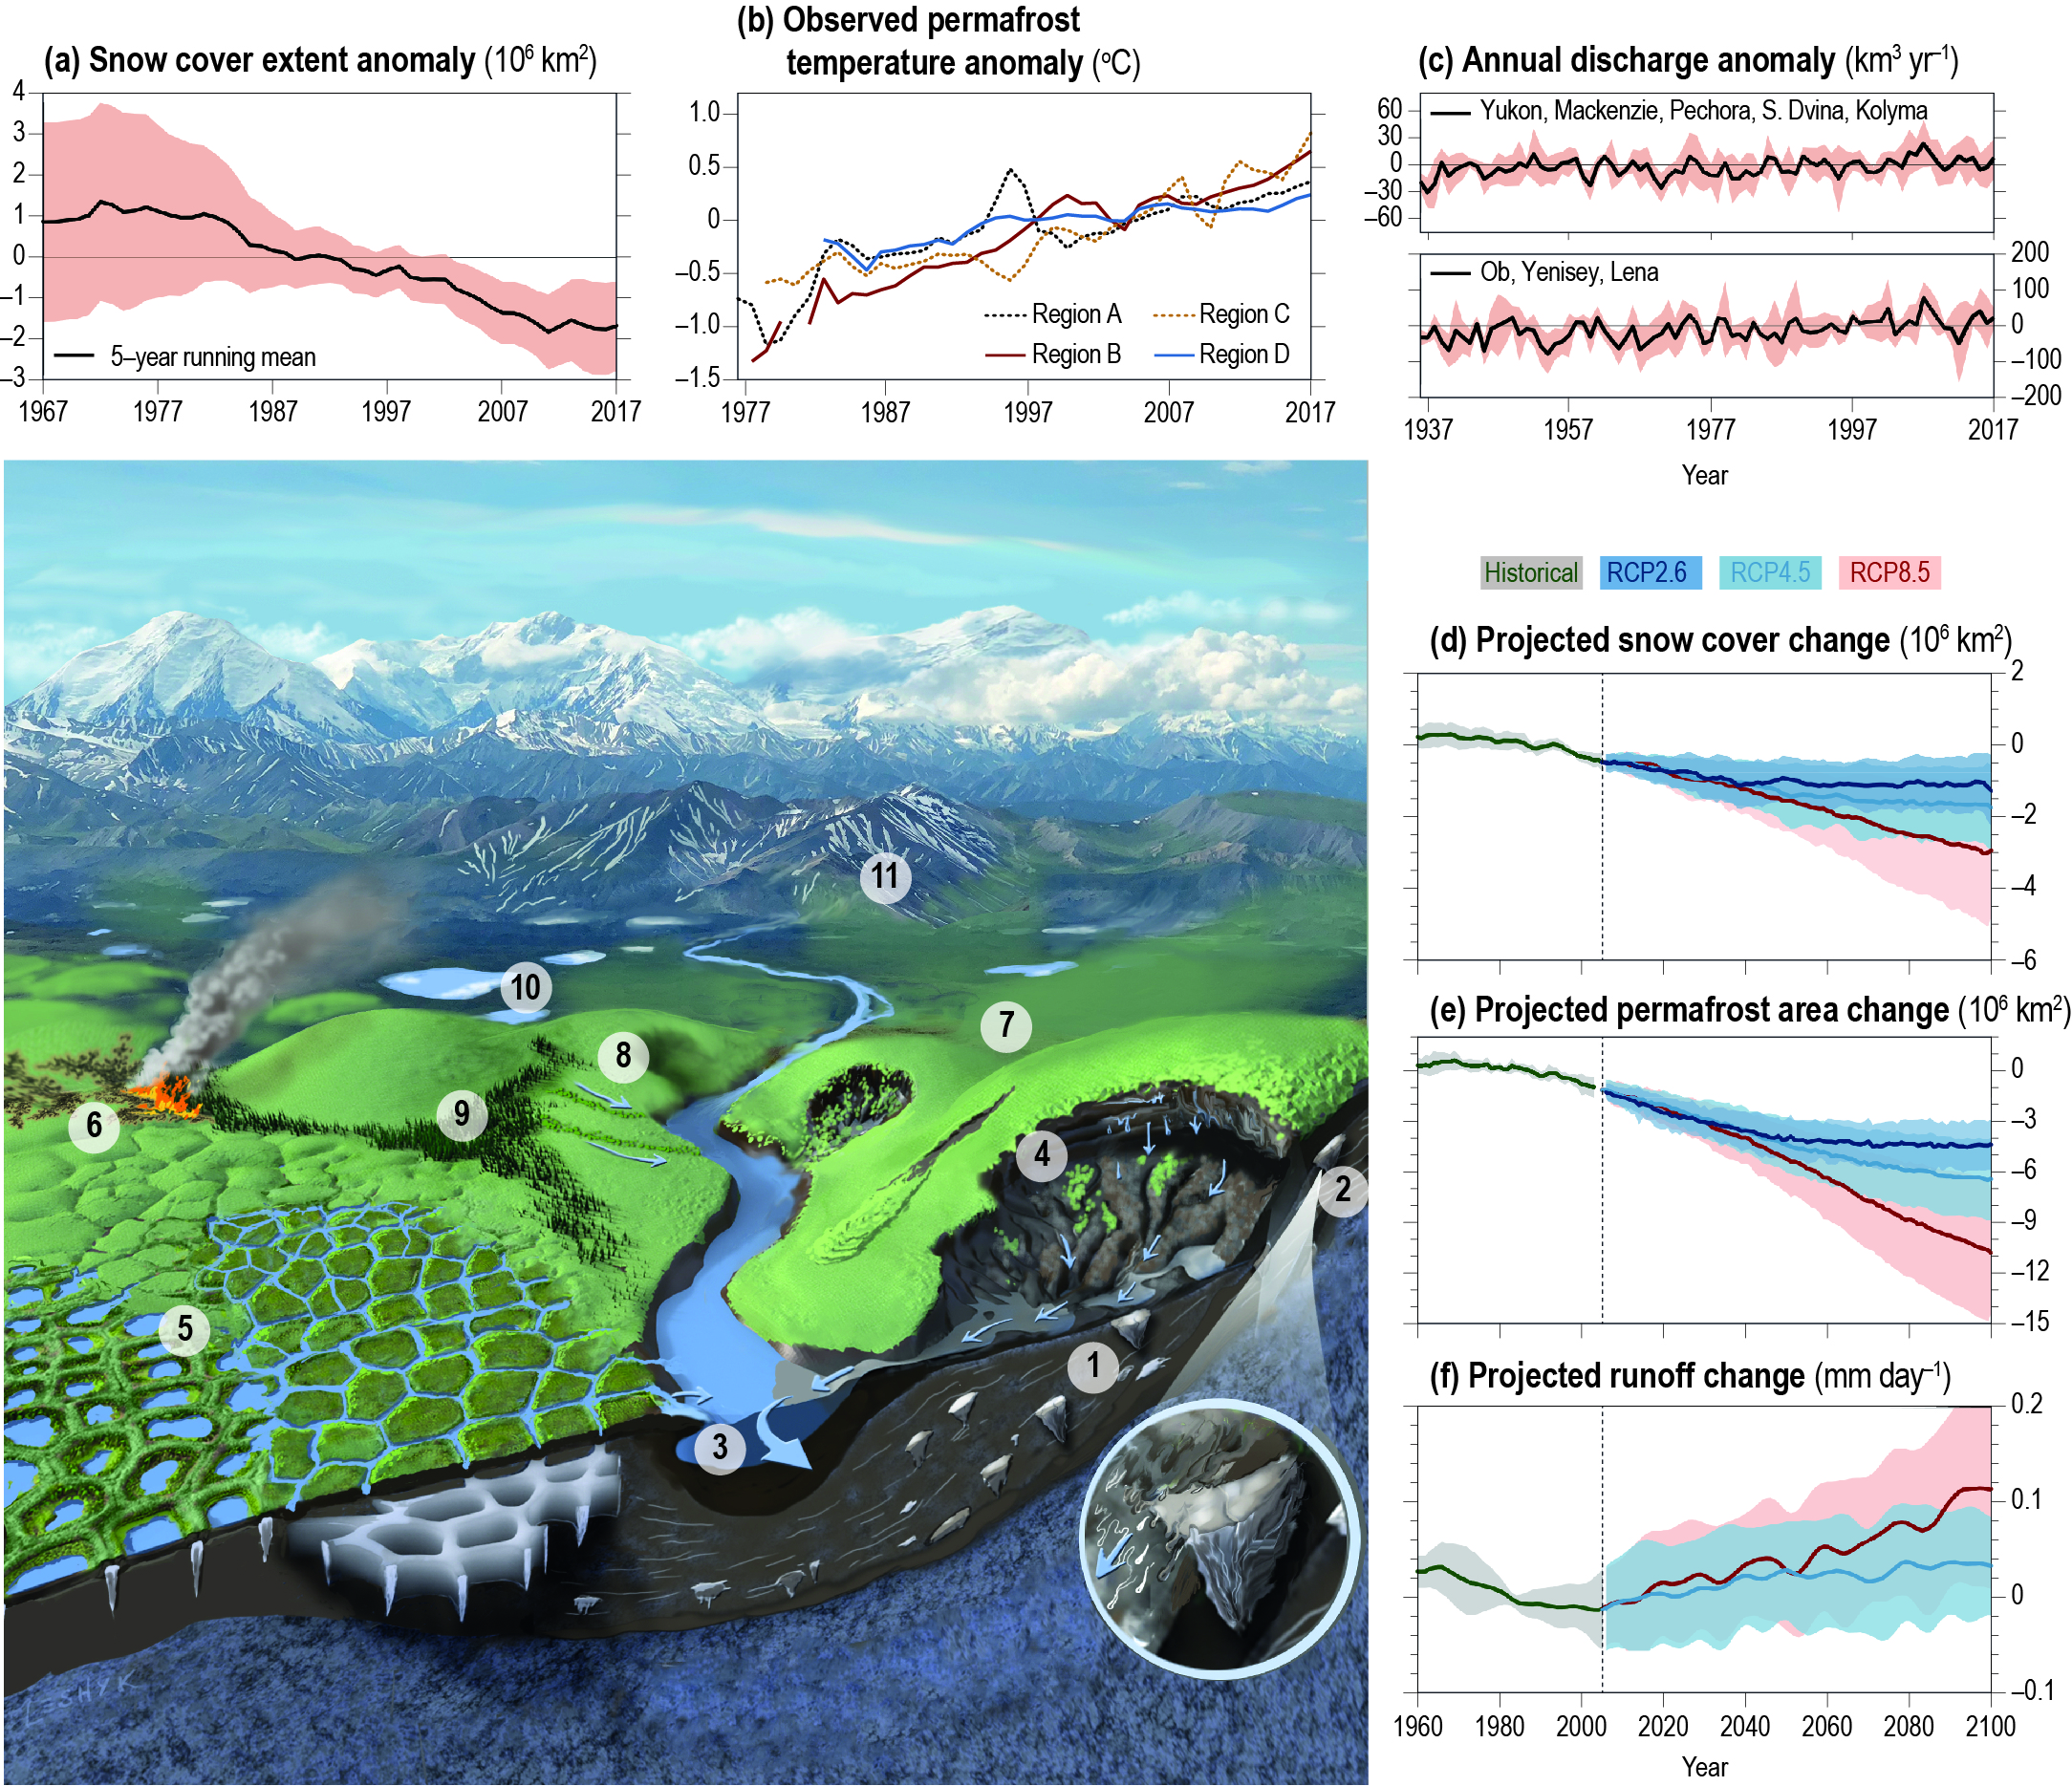
\includegraphics[width=0.9\textwidth]{IPCC-SROCC-CH_3_10.jpg}
\caption{Schematic of the important land surface components of the hydrological cycle influenced by the Arctic terrestrial cryosphere: permafrost (1); ground ice (2); river discharge (3); abrupt thaw (4); surface water (5); fire (6); tundra (7); shrubs (8); boreal forest (9); lake ice (10); seasonal snow (11). \cite{ipcc}}\label{fig:hydro}
\end{figure}

Figure \ref{fig:hydro} shows land surface components which contribute to the changing hydological cycle. Figure \ref{fig:hydro}.a is a time series of snow cover extent in June relative to 1981-2010 climatology from 5 models based on . Figure \ref{fig:hydro}.b shows the change in permafrost temperature normalised to a baseline period. Increasing permafrost temperatures result in ground instability, increased water run off and an overall increase in precipitation. Region A: Continuous to discontinuous permafrost in Scandanavia, Svalbard, and Russia/Siberia, Region B: Cold continuous permafrost in northern Alaska, Northwest Territories, and NE Siberia, Region C: Cold continuous permafrost in Eastern and High Arctic Canada, Region D: Discontinuous permafrost in Interior Alaska and Northwest Canada. Figure \ref{fig:hydro}.c shows annual runoff normalised to the 1981-2010 baseline ($\pm 1$ standard deviation. Figures \ref{fig:hydro}.d,e \& f are the Coupled Model Intercomparison Project Phase 5 (CMIP5) multi-model average (± 1 standard deviation) projections for different Representative Concentration Pathway (RCP) scenarios for d) June snow cover extent change, e) area change for near-surface permafrost and f) runoff change to the Arctic Ocean. 

Terrestrial, marine and freshwater ecosystems are strongly coupled with the cryosphere and atmosphere to form the Arctic hydrological cycle, as shown in fig.\ref{fig:hydro_cycle}.  


\begin{figure}[h!]
\centering
\includegraphics[width=0.7\textwidth]{hydological_cycle.png}
\caption{Schematic of the main freshwater components and processes in the Arctic hydrological cycle \cite{vihma2016atmospheric}. The numbers in black show the main freshwater transports in $km^3/yr$ based on \cite{serreze2006large} for 1979-2010, with the numbers in red show the estimates for 2000-2010 from   \cite{haine2015arctic}. }\label{fig:hydro_cycle}
\end{figure}


\section{Characterizing change}
Climate sensitivity 

Arctic climate change is mainly characterized by a warmer and wetter atmosphere. This is due to the overall global increase in temperature, in addition to poleward energy transport, snow and ice albedo feedbacks, loss of sea ice and snow, the confining of warming to the near-surface in the polar atmosphere, moisture transport and water-vapor radiative feedback which all contribute to amplification \cite{serreze2011processes}. These are combined effects which differ between the hemispheres.

{\color{blue}how do these changes matter and how do they differ?}

The main question and discussion regarding Arctic moistening and the increase in the overall precipitation in the region as the Arcit warms is; is the increased precipitation from local changes to the hydrological cycle (ie sea ice melt) or is it from remote sources (thus transported from lower latitudes). As explained in \cite{bintanja2014future} finding the answer to this question is important for two main reasons. The first; if the precipitation increase is largely linked to local changes, that means that the increase is due to increased warming and melt of sea ice and glaciers in the Arctic region. Since the increased melting directly contributes to increased precipitation, little changes will occur to the overall salinity of the ocean, since evaporation and precipitation will for the most part, cancel out. This is important when we think of impacts related to freshening, such as the slowing down of the AMOC. The second; if the increased precipitation is from remote changes, this means that there is an increased magnitude and frequency of merdidional transport of water vapour to the Arctic, related to more remote evaporation sources. Local and remote changes exhibit different seasonal cycles, and therefore whichever dominates will have different impacts on the local hydrology and ecology of the region.

\subsection{Humidity}\label{humidity}

Humidity is the concentration of water vapour present in the air, and depends on the temperature and pressure of the system of interest, with three measurements used. 

\subsubsection{Relative humidity}
Relative humidity, which is the ratio of partial pressure of water vapour in a mixture (ie the air) to the equilibrium vapor pressure of water over a flat surface of pure water. This measurement is the ratio of how much water vapour is in the air versus how much it could have. 

\begin{equation}
    \phi = \frac{\rho H_O}{\rho^* H_2O}
\end{equation}

where $\rho H_O$ is the partial pressure of water vapour in the mixture and $\rho^* H_O$ is the equilibrium vapour pressure of water over a flat surface of pure water. 


\subsubsection{Relative humidity}
Absolute humidity is the mass of of water vapour per unit volume of moist air or as mass of water vapour per mass of dry air, and does not take temperature into consideration.

\begin{equation}
    AH = \frac{mH_2O}{V_{net}}
\end{equation}
Where $mH_2O$ is the mass of water vapour and $V_{net}$ is the volume of air and water vapour mixture. 



\subsubsection{Specific humidity}
Specific humidity is the ratio of water vapour mass to total moist air parcel mass. It is approximately equal to the mixing ration which is  the ration of mass of water vapour in an air parcel to the mass of dry air for the same sized parcel. 



\section{Local changes}
The amount of moisture in the Arctic is determined by the rates of local evaporation and moisture transport from lower latitudes.

\subsection{Local temperature change}
mean change - more humidity 


\subsection{Local humidity change}

Humidity is the concentration of water vapour present in the air, and depends on the temperature and pressure of the system of interest, with three measurements used. 



Increasing temperature leading to how much increased humidity etc 
Temperature trend due to CC relation 

The increase in Arctic annual mean surface temperature (land and ocean) between 1971 and 2019 was three times higher than the increase in the global average during the same period \cite{AMAP}. Newer studies estimate that this change is 4 times the amount \cite{rantanen2022arctic}. These temperature increases are driving ice losses and changes in moisture transport.

show a table showing which paper, what methods, for what amount of temperature change

Moist energy balance models and general circulation models show 1.8 times more warming than dry models, due to the warming effect of latent heat transport \cite{feldl2021polar}, showing that humidity is an important factor when characterizing amplification.


\subsubsection{Clausius-Clapeyron relation}\label{cc}
The capacity of air to hold moisture increases exponentially with air temperature according to the Clausius-Clapeyron equation. Saturated water pressure P and temperature T are related as follows;

\begin{equation}
    P \propto exp\frac{-\Delta H_{vap}}{RT}
\end{equation}
where $\Delta H_{vap}$  is the Enthalpy (heat) of Vaporization and R is the gas constant. Integrating between two pressure end points gives the Clausius-Clapeyron equation;  
\begin{equation}
    ln \left ( \frac{P_1}{P_2} \right ) = \frac{\Delta H_{vap}}{R} \left ( \frac{1}{T_2} - \frac{1}{T_1} \right )
\end{equation}

This equation allows and estimate of vapour pressure at different temperatures and visa-versa, which simplifies to an increase of water retention by around $7\% / ^{\circ} C $. This would lead to a strengthening of the global evaporation (E) minus precipitation (P) pattern with overall global surface temperature increases \cite{held2006robust}. Experimental results differ from this estimation, and it has been found to have a value closer to $3.0 \pm 1.6 \% / ^{\circ} C $ from 1950 to 2010, with climate models showing an increase of $4.3 \pm 2.0 \% / ^{\circ} C $ under greenhouse gass emission scenarios \cite{Skliris2016}. 




\subsubsection{Sea ice \& Ocean interactions}
In recent years the effects of changing humidity have been explored, with the cause for overall warming being attributed to increases in humidity and precipitation \cite{mccrystall2021new} as well as sea ice losses. Humidity changes can occur both due to sea ice losses and the transport of moisture from other regions. 

how is sea ice changing humidity?
more open water for evaporation 
how do we quantify this?

how are sea ice changes affecting humidity?

increased snow changing sea ice trends


Previous work investigating Arctic amplification focused on sea ice losses \cite{serreze2009emergence}. With warming temperatures, ice has less time to form which makes it thinner and causes it to melt earlier. This allows for stronger heat transfer from the ocean to the atmosphere. There has been a considerable loss in sea ice extent since 1979, with a yearly decrease in sea ice expected to continue with the increase in CO2 in the atmosphere \cite{dai2019arctic}. 

Some work has shown that in aquaplanet models, with no sea ice, Arctic amplification still occurs \cite{russotto2020polar}, showing that while sea ice loss is an important mechanism, other factors are just as important to research when investigating what is contributing to amplification. 

As mentioned above, winter warming in the Arctic is more severe than that in the summer, with this change being attributed to sea ice changes. Sea ice changes are mainly being forced by changes in the summer climate. 
\paragraph{Ice, leads and polynas}
 Due to a large amount of evaporation from leads and polynyas, the near-surface air humidity over Arctic sea ice is generally close to saturation concerning the ice phase and therefore sublimation is weak \cite{andreas2002near}. Leads are large fractures within an expanse of sea ice, where a linear area of open water is present, and often used for transport. They can vary in width from meters to hundreds of meters. Polynyas are areas of open water surrounded by sea ice.


\subsection{Local precipitation changes}
Changes are being seen in how these sources of precipitation are changing both over time and between regions, with end-of-century humidity recycling projected to account for 60-64\% of precipitation \cite{ford2022arctic}.

overall more humidity - therefore rain instead of snow 

have this as a different paragraph??

number of events 

Changing precipitation patterns


\subsection{The influence of land interactions}
Evapotranspriation changes 
melting glaciers 

Vegetation

melting permafrost 


\section{Remote changes}
\subsection{Moisture transport and intrusions}


\subsubsection{Transported moisture}

meridional changes - differ in the summer/winter months
not much agreement here 


Other sources of atmospheric moisture in the Arctic are transported from lower latitudes, driven by the north-south gradient in air-specific humidity and are affected by large-scale circulation patterns such as planetary waves, subtropical jet stream, the Polar front jet stream and storm tracks \cite{gimeno2019atmospheric}. These phenomena are split up into mean meridional circulation, stationary eddies and transient eddies. 

There has been an overall increase in atmospheric and ocean heat transport to the poles due to changes in the transport of latent energy (moisture) and dry static energy (the sum of sensible and potential energy) by atmospheric circulations \cite{mcgraw2020changes}. Particularly there are large increases seen over the Atlantic sector of the Arctic \cite{dufour2016atmospheric}, with little analysis of moisture transport over the Western Canadian Arctic. 

\subsection{Storm tracks and blocking}
\subsection{Aerosols}
see figure 1 \cite{vihma2016atmospheric}
\section{Knowledge gaps}
\section{Conclusion}






 \bibliography{../mybib}{}
\bibliographystyle{apalike}

\end{document}


